\documentclass[ja=minimal]{bxjsarticle}
\usepackage{tikz}
\usepackage{luatexja}
\usepackage{luatexja-fontspec}


\usepackage{pgfplots}
\usepackage{amsmath}
\pgfplotsset{compat=1.18}
\usepackage{graphicx}
\usepackage{multicol}
\usetikzlibrary{intersections,calc,arrows.meta,angles,quotes,patterns}
\usepgfplotslibrary{fillbetween}

\begin{document}

\begin{center}
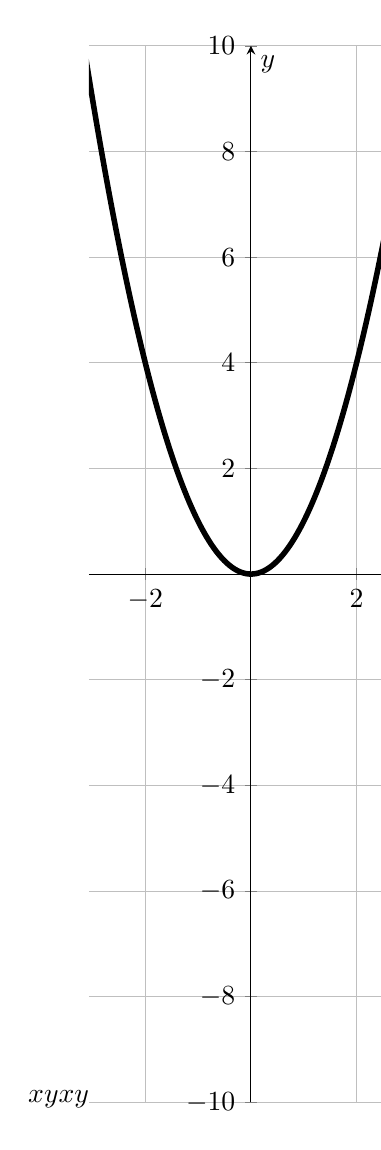
\begin{tikzpicture}

\pgfmathsetmacro{\a}{1.0}

\pgfmathsetmacro{\b}{2.0}
\begin{axis}[
            width=15cm,
            height=15cm,
            axis equal image,
            axis lines=middle,
            grid=major,
            enlargelimits=false,
            clip=true,
            xlabel=$x$,
            ylabel=$y$,
            domain=-10.0:10.0,
            ymin=-10.0,ymax=10.0,
            view={0}{90},
            samples=200
            ]
        

            width=15cm,
            height=15cm,
            axis equal image,
            axis lines=middle,
            grid=major,
            enlargelimits=false,
            clip=true,
            xlabel=$x$,
            ylabel=$y$,
            domain=-10.0:10.0,
            ymin=-10.0,ymax=10.0,
            view={0}{90},
            samples=200
            ]
        

            width=15cm,
            height=15cm,
            axis equal image,
            axis lines=middle,
            grid=major,
            enlargelimits=false,
            clip=true,
            xlabel=$x$,
            ylabel=$y$,
            domain=-10.0:10.0,
            ymin=-10.0,ymax=10.0,
            view={0}{90},
            samples=200
            ]
        
\addplot[samples=200, smooth, line width=2pt, black, variable=x] {x^2};
\end{axis}
\end{tikzpicture}
\end{center}

\end{document}
